\documentclass{beamer}
\usepackage[utf8]{inputenc}

\usetheme{Madrid}
\usecolortheme{default}
\usepackage{amsmath,amssymb,amsfonts,amsthm}
\usepackage{txfonts}
\usepackage{tkz-euclide}
\usepackage{listings}
\usepackage{adjustbox}
\usepackage{array}
\usepackage{tabularx}
\usepackage{gvv}
\usepackage{lmodern}
\usepackage{circuitikz}
\usepackage{tikz}
\usepackage{graphicx}
 \graphicspath{{figs/}}
\setbeamertemplate{page number in head/foot}[totalframenumber]
\usepackage[T1]{fontenc}
\usepackage{lmodern}

\usepackage{tcolorbox}
\tcbuselibrary{minted,breakable,xparse,skins}



\definecolor{bg}{gray}{0.95}
\DeclareTCBListing{mintedbox}{O{}m!O{}}{%
  breakable=true,
  listing engine=minted,
  listing only,
  minted language=#2,
  minted style=default,
  minted options={%
    linenos,
    gobble=0,
    breaklines=true,
    breakafter=,,
    fontsize=\small,
    numbersep=8pt,
    #1},
  boxsep=0pt,
  left skip=0pt,
  right skip=0pt,
  left=25pt,
  right=0pt,
  top=3pt,
  bottom=3pt,
  arc=5pt,
  leftrule=0pt,
  rightrule=0pt,
  bottomrule=2pt,
  toprule=2pt,
  colback=bg,
  colframe=orange!70,
  enhanced,
  overlay={%
    \begin{tcbclipinterior}
    \fill[orange!20!white] (frame.south west) rectangle ([xshift=20pt]frame.north west);
    \end{tcbclipinterior}},
  #3,
}
\lstset{
    language=C,
    basicstyle=\ttfamily\small,
    keywordstyle=\color{blue},
    stringstyle=\color{orange},
    commentstyle=\color{green!60!black},
    numbers=left,
    numberstyle=\tiny\color{gray},
    breaklines=true,
    showstringspaces=false,
}
%------------------------------------------------------------
%This block of code defines the information to appear in the
%Title page
\title %optional
{1.8.24}
%\subtitle{A short story}

\author % (optional)
{Aniket-EE25BTECH11007}

\begin{document}
\frame{\titlepage}
\begin{frame}{Question}
If $\vec a$ and $\vec b$ are unit vectors, find the angle $\theta$ between $\vec a$ and $\vec b$
such that $\vec a-\sqrt{2}\,\vec b$ is a unit vector.\\
\end{frame}

\begin{frame}{Theoretical Solution}
    Since $\vec a$ and $\vec b$ are unit vectors,
\begin{gather}
\lVert \vec a \rVert = 1 \label{eq:unit-a}\\
\lVert \vec b \rVert = 1 \label{eq:unit-b}
\end{gather}
The condition that $\vec a-\sqrt{2}\,\vec b$ is also a unit vector gives
\begin{equation}
\big\lVert \vec a-\sqrt{2}\,\vec b \big\rVert = 1.
\label{eq:unit-cond}
\end{equation}
Squaring both sides:
\begin{equation}
\big\lVert \vec a-\sqrt{2}\,\vec b\big\rVert^{2}
= (\vec a-\sqrt{2}\,\vec b)^{\top}(\vec a-\sqrt{2}\,\vec b)=1.
\label{eq:norm-squared}
\end{equation}

\end{frame}

\begin{frame}{Theoretical Solution}
    \begin{equation}
(\vec a-\sqrt{2}\,\vec b)^{\top}(\vec a-\sqrt{2}\,\vec b)
= \vec a^{\top}(\vec a-\sqrt{2}\,\vec b)
\;-\;\sqrt{2}\,\vec b^{\top}(\vec a-\sqrt{2}\,\vec b).
\label{eq:distribute-outer}
\end{equation}

Using \eqref{eq:unit-a} and \eqref{eq:unit-b} and $\vec a^{\top}\vec b=\vec b^{\top}\vec a$:
\begin{equation}
1=(\vec a-\sqrt{2}\,\vec b)^{\top}(\vec a-\sqrt{2}\,\vec b)
= 1 -\sqrt{2}\,\vec a^{\top}\vec b \;-\;\sqrt{2}\,\vec a^{\top}\vec b \;+\;2
= 3 - 2\sqrt{2}\,(\vec a^{\top}\vec b).
\label{eq:combine}
\end{equation}

\begin{equation}
2\sqrt{2}\,(\vec a^{\top}\vec b)=2
\;\Longrightarrow\;
\vec a^{\top}\vec b=\frac{1}{\sqrt{2}}.
\label{eq:atb}
\end{equation}
\end{frame}

\begin{frame}{Theoretical Solution}
    Using the angle formula from dot product,
\begin{equation}
\cos\theta=\frac{\vec a^{\top}\vec b}{\lVert\vec a\rVert\,\lVert\vec b\rVert}
=\frac{1/\sqrt{2}}{1\cdot 1}=\frac{1}{\sqrt{2}},
\label{eq:costheta}
\end{equation}

\begin{equation}
\boxed{\;\theta=\frac{\pi}{4}=45^\circ\;}
\label{eq:final}
\end{equation}
\end{frame}

\begin{frame}[fragile]
    \frametitle{C Code }

    \begin{lstlisting}
#include <math.h>
#include <stdio.h>

int solve_angle_simple(const double *a, const double *b, int n, double *theta_deg) {
    const double SQRT2 = 1.4142135623730950488;
    const double PI    = 3.14159265358979323846;
    const double TOL   = 1e-9;

    double aa = 0.0, bb = 0.0, lhs_sq = 0.0;
    for (int i = 0; i < n; ++i) {
        aa += a[i] * a[i];
        bb += b[i] * b[i];
        double t = a[i] - SQRT2 * b[i];
        lhs_sq += t * t;
    }
    double na = sqrt(aa);
    double nb = sqrt(bb);
    double lhs = sqrt(lhs_sq);
        \end{lstlisting}
\end{frame}
\begin{frame}[fragile]
    \frametitle{C Code }

    \begin{lstlisting}
    double ab = 0.0;
    for (int i = 0; i < n; ++i) ab += a[i] * b[i];

    double denom = na * nb;
    double cos_theta = (denom > 0.0) ? (ab / denom) : 1.0;
    if (cos_theta >  1.0) cos_theta =  1.0;
    if (cos_theta < -1.0) cos_theta = -1.0;
    *theta_deg = acos(cos_theta) * (180.0 / PI);

    if (fabs(na - 1.0) <= TOL && fabs(nb - 1.0) <= TOL && fabs(lhs - 1.0) <= TOL) {
        *theta_deg = 45.0;
        return 0;
    }
    return 1;
}

    \end{lstlisting}
\end{frame}
\begin{frame}[fragile]
    \frametitle{Python+C Code}
    \begin{lstlisting}
import ctypes
from ctypes import c_double, c_int
import numpy as np
import matplotlib.pyplot as plt

# --- load the shared lib ---
# Change name below if you're on macOS (.dylib) or Windows (.dll)
lib = ctypes.CDLL("./mg3.so")

# C signature:
# int solve_angle_simple(const double *a, const double *b, int n, double *theta_deg)
lib.solve_angle_simple.argtypes = [
    ctypes.POINTER(c_double),
    ctypes.POINTER(c_double),
    c_int,
    ctypes.POINTER(c_double),
]
lib.solve_angle_simple.restype = c_int
  \end{lstlisting}
    \end{frame}
    \begin{frame}[fragile]
    \frametitle{Python+C Code}
    \begin{lstlisting}
def solve_angle_np(a: np.ndarray, b: np.ndarray):
    """
    Call the C function using NumPy arrays a, b (1D, same length).
    Returns (theta_deg, status) where status==0 if the unit checks passed.
    """
    a = np.asarray(a, dtype=np.float64).ravel()
    b = np.asarray(b, dtype=np.float64).ravel()
    if a.shape != b.shape:
        raise ValueError("a and b must have the same shape")

    theta = c_double(0.0)
    pa = a.ctypes.data_as(ctypes.POINTER(c_double))
    pb = b.ctypes.data_as(ctypes.POINTER(c_double))
    status = lib.solve_angle_simple(pa, pb, a.size, ctypes.byref(theta))
    return theta.value, status
 \end{lstlisting}
    \end{frame}
    \begin{frame}[fragile]
    \frametitle{Python+C Code}
    \begin{lstlisting}
def plot_vectors(a: np.ndarray, b: np.ndarray, theta_deg: float):
    """Plot a, b, and a - √2 b on the unit circle for context."""
    a = np.asarray(a, dtype=np.float64).ravel()
    b = np.asarray(b, dtype=np.float64).ravel()
    c = a - np.sqrt(2.0) * b

    # 2D only for plotting
    if a.size != 2:
        raise ValueError("Plot expects 2D vectors (length 2).")

    # unit circle
    t = np.linspace(0, 2*np.pi, 400)
    plt.figure(figsize=(6,6))
    plt.plot(np.cos(t), np.sin(t), label="Unit circle")
 \end{lstlisting}
    \end{frame}
    \begin{frame}[fragile]
    \frametitle{Python+C Code}
    \begin{lstlisting}
    # vectors
    plt.quiver(0,0, a[0], a[1], angles='xy', scale_units='xy', scale=1, label="a")
    plt.quiver(0,0, b[0], b[1], angles='xy', scale_units='xy', scale=1, label="b")
    plt.quiver(0,0, c[0], c[1], angles='xy', scale_units='xy', scale=1, label="a − √2 b")

    # angle arc (between a and b) if both unit and 2D
    theta = np.deg2rad(theta_deg)
    arc = np.linspace(0, theta, 100)
    plt.plot(0.25*np.cos(arc), 0.25*np.sin(arc))
    plt.text(0.32*np.cos(theta/2), 0.32*np.sin(theta/2), rf"$\theta={theta_deg:.0f}^\circ$")

    plt.gca().set_aspect('equal', adjustable='box')
    plt.grid(True, linewidth=0.4, alpha=0.5)
    plt.xlim(-1.6, 1.6); plt.ylim(-1.6, 1.6)
    plt.legend()
     \end{lstlisting}
    \end{frame}
    \begin{frame}[fragile]
    \frametitle{Python+C Code}
    \begin{lstlisting}
    plt.title("Vectors a, b, and a − √2 b")
    plt.tight_layout()
    plt.show()

if __name__ == "__main__":
    # Example: a is x-axis unit; b is unit at 45°
    a = np.array([1.0, 0.0])
    b = np.array([np.cos(np.pi/4), np.sin(np.pi/4)])

    theta_deg, status = solve_angle_np(a, b)
    print(f"theta from C = {theta_deg:.6f}°, status={status} (0 means unit checks passed)")
    print(f"||a||={np.linalg.norm(a):.3f}, ||b||={np.linalg.norm(b):.3f}, "
          f"||a-√2 b||={np.linalg.norm(a - np.sqrt(2)*b):.3f}")

    plot_vectors(a, b, theta_deg)

    \end{lstlisting}
    \end{frame}


    \begin{frame}[fragile]
    \frametitle{Python Code}
    \begin{lstlisting}
import numpy as np
import matplotlib.pyplot as plt

# --- choose 2D unit vectors (you can edit these) ---
theta_true = np.deg2rad(45)           # 45°
a = np.array([1.0, 0.0])              # unit along +x
b = np.array([np.cos(theta_true), np.sin(theta_true)])  # unit at 45°

# --- compute angle θ (in degrees) ---
dot = float(np.dot(a, b))
na  = float(np.linalg.norm(a))
nb  = float(np.linalg.norm(b))
cos_theta = dot / (na * nb)
cos_theta = max(-1.0, min(1.0, cos_theta))  # clamp for safety
theta_deg = float(np.degrees(np.arccos(cos_theta)))
    \end{lstlisting}
    \end{frame}
    \begin{frame}[fragile]
    \frametitle{Python Code}
    \begin{lstlisting}
# --- check the condition ||a||=||b||=||a-√2 b||=1 ---
c = a - np.sqrt(2.0) * b
print(f"θ = {theta_deg:.2f}°,  ||a||={na:.2f}, ||b||={nb:.2f}, ||a-√2 b||={np.linalg.norm(c):.2f}")

# --- plot unit circle + vectors ---
t = np.linspace(0, 2*np.pi, 400)
plt.figure(figsize=(6,6))
plt.plot(np.cos(t), np.sin(t), label="Unit circle")
plt.quiver(0,0, a[0], a[1], angles='xy', scale_units='xy', scale=1, label="a")
plt.quiver(0,0, b[0], b[1], angles='xy', scale_units='xy', scale=1, label="b")
plt.quiver(0,0, c[0], c[1], angles='xy', scale_units='xy', scale=1, label="a − √2 b")
\end{lstlisting}
    \end{frame}
    \begin{frame}[fragile]
    \frametitle{Python Code}
    \begin{lstlisting}
# angle arc (purely for illustration)
arc = np.linspace(0, np.deg2rad(theta_deg), 100)
plt.plot(0.25*np.cos(arc), 0.25*np.sin(arc))
plt.text(0.32*np.cos(np.deg2rad(theta_deg)/2),
         0.32*np.sin(np.deg2rad(theta_deg)/2),
         rf"$\theta={theta_deg:.0f}^\circ$")

plt.gca().set_aspect('equal', adjustable='box')
plt.grid(True, linewidth=0.4, alpha=0.5)
plt.xlim(-1.6, 1.6); plt.ylim(-1.6, 1.6)
plt.legend(); plt.title("a, b, and a − √2 b"); plt.tight_layout()
plt.show()

    \end{lstlisting}
    \end{frame}


\begin{frame}{Plot}
    \begin{figure}[H]
    \centering
    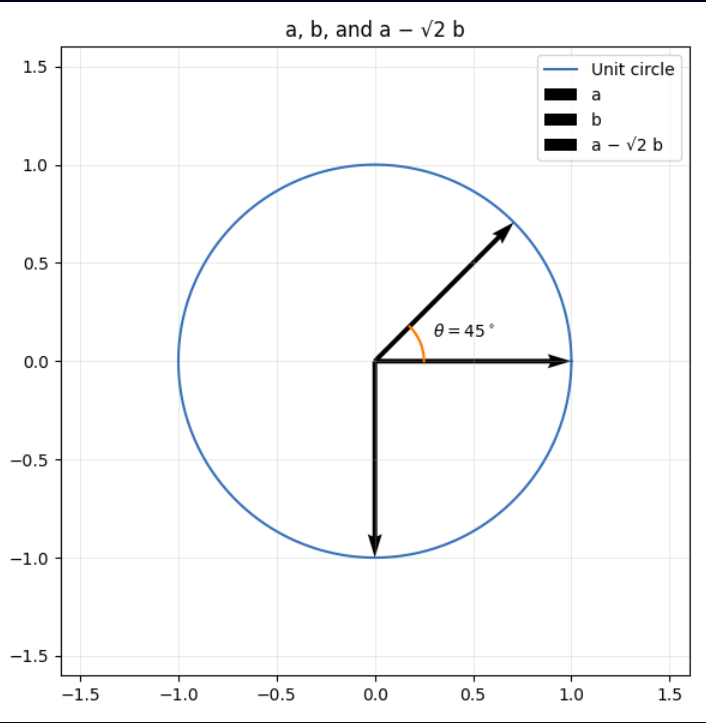
\includegraphics[width=0.65\columnwidth]{figs/mg3plot.png}
\end{figure}
\end{frame}
\end{document}